\chapter{Preliminaries}
\section{Biological entities and their analysis}

%When we think about biology, we first picture living organisms, the basic unit of biology.
%Living organisms are very diverses, ranging from higher animals, mammals and vertebrates, to microorganisms, bacteria and some fungi.
%Yet as diverse as organisms may be, they are all made of the same biological entity: the cell.
%
%Cells are the simplest constituents of the living : they are self-organizing complex systems that can replicate, grow, and adapt to their environement in order to maintain the stability of their internal processes \parencites{mckay2004life}{trifonov2012author}.
%Cells are divided into two types, the prokaryotic cells that compose unicellular organisms (such as bacteria), and the eukaryotic cells that compose multicellular organisms (such as animals).
%The main structural difference between prokaryotic and eukaryotic cells is the presence of a nucleus in the latter, that encloses and protect most of the genetic information of the organism.
%
%This genetic material is at the foundation of every known living organism \parencite{raven2013biology}, and at the biomolecular level is composed of Deoxyribonucleic Acid (DNA) molecules.
%DNA modules are long stranded molecules that encode the necessary instructions to create the functionnal components of a cell, and all different DNA molecules of an organisms are called its genome.
%The sections of the genome that encore the instructions, the coding regions, are the genes.
%
%From DNA molecules, two types of information transfer can occur: \emph{DNA replication} that creates a copy of the molecule, and \emph{transcription} that creates a messenger RNA molecule from a gene.
%Messenger RNA (mRNA) molecules are Ribonucleic acid (RNA) molecules that are used as templates by the cellular machinery to create proteins during the \emph{translation} process.
%
%The \emph{central dogma of molecular biology} states that information transfer can only occur in this order, from DNA to RNA, and from RNA to proteins \parencite{crick1970central}.
%
%Proteins are large molecules organized in one of more, possibly folded, chain of amino acids compounds.
%Each cell contains a very wide variety of proteins, and together they all constitute its molecular machinery.

We first briefly overview the types of information that is available to study biological systems.
This information can be described following the \emph{central dogma of molecular biology} \parencite{crick1970central}: genetic (DNA) sequences, transcribed RNA sequences and finally protein sequences.
Raw DNA sequences are strings of the four letters, called \emph{bases}, comprising genes. Different species can have different numbers of genes within the genome of the organism.
For prokaryotes, each gene is typically $1,000$ to $2500$ bases long \parencite{xu2006average}.
The GenBank repository of nucleic acid sequences (\url{http://www.ncbi.nlm.nih.gov/genbank/}) currently holds a total of approximately 202 billion bases in 188 million entries\footnote{Release 210.0, October 15 2015}.
At the next level are protein sequences that correspond to real gene products within the cells and are strings of 21 amino acid-letters.
At present, the UniProtKB protein sequence database (\url{http://www.uniprot.org/}) contains about 500 thousands reviewed protein sequences\footnote{Release 2015\_10}, a typical bacterial protein being approximately 300 amino acids long.

The central dogma states that DNA makes RNA, and RNA makes proteins.
At each step, a cell translates the information between the different alphabets.
That is, DNA sequences are translated into RNA sequences at the first step, and RNA sequences are translated into protein sequences at the second step, see \cref{fig:centraldogma}.

\begin{figure}[ht]
\centering
\begin{tikzpicture}[
    >=latex,thick,
    /pgf/every decoration/.style={/tikz/sharp corners},
    minimum size=6mm,line join=round,line cap=round,
    terminal/.style={rectangle,draw,rounded corners=1mm},
    %node distance=4cm
  ]

    \begin{scope}[start chain,
            every node/.style={on chain},
            terminal/.append style={join=by {->,shorten >=-1pt,
                decoration={post length=4pt}}}
        ]
        \node [terminal] (dna)                     {DNA};
        \node [terminal] (rna)  [right=3cm of dna] {RNA};
        \node [terminal] (prot) [right=3cm of rna] {protein};
    \end{scope}
    \node (exdna)  [below=of dna]  {ACCCATAGTCGC\ldots{}};
    \node (exrna)  [below=of rna]  {ACCCAUAGUCGC\ldots{}};
    \node (exprot) [below=of prot] {MAQW\ldots{}};
\end{tikzpicture}
\caption[Central Dogma of Biology]{\textbf{Central Dogma of Molecular Biology.} Below each structure type are examples using 12 dummy DNA characters, the corresponding messenger RNA sequence, and the protein sequence.}
\label{fig:centraldogma}
\end{figure}

\subsection{Entities}

\subsubsection{Genes}

%Every cell of a given organism share the exact same genome.
%Each gene can be represented as a Deoxyribonucleic acid (DNA) sequence. There exists four DNA molecules: 
A genome is typically a set of sequences, corresponding to chromosomes, over the 4-letter alphabet: cytosine ('C'), guanine ('G'), adenine ('A'), and thymine ('T'). The set of genes of an organism encodes the instructions for a cell to perform its functions. In order to study how cells perform their functions, it is first necessary to identify genes. Process of identifying regions within the genome that encode genes is called \emph{gene finding}, see for review \parencite{stormo2000gene}. The common principle behind gene prediction methods is to distinguish between protein-coding regions (genes) and non-coding regions, based on their statistical properties.

%Genomics is the field that study the functions and structure of genomes.

%Thus, genes can be represented as a sequence of DNA over the alphabet {C,G,A,T}.

\begin{figure}[ht]
  \centering
  \begin{SaveVerbatim}{STAT3}
CGGGGTTAAATCCACTACCCTCTCCCCACGCACTC
TAGTAATTACTCTATTTCCACGTCATGTTTCCGGG
\end{SaveVerbatim}
  \BUseVerbatim{STAT3}
  \caption{70 nucleobases from the human (hsa) STAT3 gene.}
\end{figure}

%\TODO{DNA is obtained by sequencing ; whole genome / exome}

Based on the observation that given two species $A$ and $B$, there exist gene versions $a \in A$ and $b \in B$ that are similar in sequence and have related functions, the parsimony principle suggests that they must have been inherited from the common ancestor. Genes that have a  \emph{similar sequence} are said to be \emph{homologs}. Among homologs there are two main subgoups: orthologs and paralogs. \emph{Orthologs} are homologous genes that evolved from the same ancestral gene in the last common ancestor of the compared species. For example, for $a$ and $b$ to be orthologs, they must have descended from an ancestral gene $c$ in $C$, last common ancestor of $A$ and $B$. On the other hand, \emph{paralogs} are homologous genes, that have evolved by duplication. For example, $a' \in A$ having a similar sequence to $a$ (and $b$), might have descended from the duplication of $a$ that has happened after the ancestors of $A$ and $B$ have taken different evolutionary paths. For further discussion of orthology, see \parencites{makarova2007clusters}{kuzniar2008quest}.


\begin{figure}[ht]
  \centering
  \begin{SaveVerbatim}[commandchars=\\\{\},codes={\catcode`$=3\catcode`^=7\catcode`_=8}]{Stat3}
CCGGGTTA\textcolor{red}{T}A\textcolor{red}{G}CCACTA\textcolor{red}{TT}CTC\textcolor{red}{-}CCCCACGCAATC
TAGTAATTACTCTATTTCCACGTCAT\textcolor{red}{A}TTTCCGGG
\end{SaveVerbatim}
  \BUseVerbatim{Stat3}
  \caption[70 nucleobases from the mouse (mus) Stat3 gene.]{70 nucleobases from the mouse (mus) Stat3 gene. Bases highlighted in \textcolor{red}{red} indicate a variation from the corresponding bases in the human gene, '-' indicates that the base is abscent in the mouse gene.}
\end{figure}

%Two genes are said homologous if they share a common ancestry preserved through evolutionary processes. (homology vs orthology ?)

%REFS (orthology) : \parencites{makarova2007clusters}{kuzniar2008quest}

\subsubsection{RNA}

Like DNA, RNA is a nucleic acid sequence, but with some differences. For example, RNA molecules are single-stranded, while DNA is double-stranded. Also DNA and RNA differ slightly at the nucleotide level, in particular there is a 'U' (uracil) instead of 'T'. Most importantly, RNA sequences ---called mRNA for messenger RNA--- correspond to the protein coding regions. %The non-coding regions are excised during the transcription process.

%copy the example : http://jonlieffmd.com/wp-content/uploads/2012/12/splicing1.gif
\colorlet{ColorPink}{red!17}
\colorlet{ColorBlue}{blue!19}
\colorlet{ColorGreen}{green!22}
\colorlet{ColorGray}{gray!22}
\begin{figure}[ht]
\centering
\footnotesize
\makebox[0pt]{
\begin{tikzpicture}[
      start chain=1 going right,start chain=2 going right,node distance=0mm,
      every node/.style={inner sep=1pt, line width=0cm},
      primer/.style={fill=ColorPink,on chain=1},
      exon/.style={fill=ColorGray,on chain=1},
      intron/.style={fill=ColorGreen,on chain=1},
      %startcodon/.style={fill=ColorBlue,on chain=2},
      startcodon/.style={fill=ColorGray,on chain=2},
      rnaexon/.style={fill=ColorGray,on chain=2},
      rnaintron/.style={fill=ColorGreen,on chain=2}
    ]

    \foreach \x in {A,C,G,T,C,T,A} {
      \node [primer] {\x};
    }

    \node [exon] (exon11) {G};
    \foreach \x in {T,A} {
      \node [exon] {\x};
    }
    \node [exon] (exon12) {C};
    \node [exon] (exon13) {T};
    \foreach \x in {G,C,A,T} {
      \node [exon] {\x};
    }
    \node [exon] (exon14) {T};

    \node [intron] (intron11) {A};
    \foreach \x in {G,C,G,A,T} {
      \node [intron] {\x};
    }
    \node [intron] (intron12) {G};

    \node [exon] (exon21) {C};
    \foreach \x in {A,T,A,C} {
      \node [exon] {\x};
    }
    \node [exon] (exon22) {G};

    \node [intron] (intron21) {A};
    \foreach \x in {T,G,C,A,T,G,C,A,A} {
      \node [intron] {\x};
    }
    \node [intron] (intron22) {A};

    \node [exon] (exon31) {G};
    \foreach \x in {G,C,A,T,A} {
      \node [exon] {\x};
    }
    \node [exon] (exon32) {C};

    \node at (3.75,-1) [startcodon] (startcodon1) {G};
    \foreach \x in {U,A} {
      \node [startcodon] {\x};
    }
    \node [startcodon] (startcodon2) {C};

    \node [rnaexon] (rnaexon11) {U};
    \foreach \x in {G,C,A,U} {
      \node [rnaexon] {\x};
    }
    \node [rnaexon] (rnaexon12) {U};
   %\foreach \x in {A,G,C,G,A,U,G} {
   %  \node [rnaintron] {\x};
   %}
    \node [rnaexon] (rnaexon21) {C};
    \foreach \x in {A,U,A,C} {
      \node [rnaexon] {\x};
    }
    \node [rnaexon] (rnaexon22) {G};
   %\foreach \x in {A,U,G,C,A,U,G,C,A,A,A} {
   %  \node [rnaintron] {\x};
   %}
    \node [rnaexon] (rnaexon31) {G};
    \foreach \x in {G,C,A,U,A} {
      \node [rnaexon] {\x};
    }
    \node [rnaexon] (rnaexon32) {C};

    \draw [black]   (exon11.south west) -- (exon11.north west);
    %\draw [red]   (exon12.south east) -- (exon12.north east);
    %\draw [black] (exon13.south west) -- (exon13.north west);
    \draw [black] (exon14.south east) -- (exon14.north east);
    \draw [black] (exon21.south west) -- (exon21.north west);
    \draw [black] (exon22.south east) -- (exon22.north east);
    \draw [black] (exon31.south west) -- (exon31.north west);
    \draw [black] (exon32.south east) -- (exon32.north east);

    \draw [black]   (startcodon1.south west) -- (startcodon1.north west);
    %\draw [red]   (startcodon2.south east) -- (startcodon2.north east);
    %\draw [black] (rnaexon11.south west) -- (rnaexon11.north west);
    \draw [black] (rnaexon12.south east) -- (rnaexon12.north east);
    %\draw [black] (rnaexon21.south west) -- (rnaexon21.north west);
    \draw [black] (rnaexon22.south east) -- (rnaexon22.north east);
    %\draw [black] (rnaexon31.south west) -- (rnaexon31.north west);
    \draw [black] (rnaexon32.south east) -- (rnaexon32.north east);

    \draw [black] (exon11.south west) -- (startcodon1.north west);
    %\draw [red] (exon12.south east) -- (startcodon2.north east);
    %\draw [black] (exon13.south west) -- (rnaexon11.north west);
    \draw [black] (exon14.south east) -- (rnaexon12.north east);
    \draw [black] (exon21.south west) -- (rnaexon21.north west);
    \draw [black] (exon22.south east) -- (rnaexon22.north east);
    \draw [black] (exon31.south west) -- (rnaexon31.north west);
    \draw [black] (exon32.south east) -- (rnaexon32.north east);
\end{tikzpicture}
}
\caption[Gene transcription]{\textbf{Gene transcription.} After the removal of the \emph{primer} region, which indicates the start of a gene, each \emph{exon} is translated by replacing every Thymine base by an Uracil base.}
\label{fig:transcription}
\end{figure}


Different species have their own sets of mRNA sequences at any given  time. In particular, they respond to environmental stimuli by varying the level of mRNA molecules that are present at a given time, process that is called \emph{gene expression}. The set of mRNA molecules of an organism is called \emph{transcriptome}.

%\TODO{RNA is obtained by sequencing, captures the expression of exome}

\subsubsection{Proteins}

\emph{Translation}, which is the second step in gene expression, ''reads'' the RNA sequences and translates (according to the genetic code) them into amino acid sequences, that is sequences over the alphabet of 21 amino-acid letters.  Each group of three bases in the mRNA constitutes a  \emph{codon}, and each codon defines a particular amino acid. This is why it is called a triplet code. Consequently, the mRNA sequence is used as a template to build sequences of amino acids that constitute proteins.

%\TODO{example of a protein}

%\TODO{Proteins are measured by ... but can be obtained by sequencing (peptides)}

\subsection{Biology as data science}

%The completion of the first sequencing projects led to many genetic insights.
%Further, s

Since the completion of the Human Genome Project in 2003, thousands of species have seen their genome fully sequenced \parencite{reddy2014genomes}.
Nowadays, \textcite{regalado2014emtech} estimated that our sequencing capacity exceeds 35 Petabases (or approximately 250,000 human genomes) per year.
Looking into the future, with further advancement of high-throughput sequencing technologies, the prospect of seeing more than 1 billion genomes sequenced in the next 20 years is  realistic \parencite{schatz2015biological}.

Genetic information is only one type of data.
In the last 20 years, many techniques have been used to look deeper into  cellular functions.
Microarrays, RNA-sequencing, high precision microscopy, and mass spectrometry, all allow automated collection of observations of the cellular developments and regulation processes.

With the collection of these volumes of data, a number of challenges arise, among which (i) the collection of data  into accessible repositories, and (ii) the analysis and interpretation of the underlying knowledge.
Analysis requirements of biological data have brought  biology within the scope of data science, towards what is called quantitative biology.

%\subsubsection{Biological databases}


\subsection{High throughput experiments}

%\subsubsection{microarrays}

This ability to quantify many molecular targets in parallel was an important step towards the understanding of complex biological processes.
\emph{Microarrays} is an experimental technique that can analyze the expression of many genes simultaneously and in an efficient manner \parencites{smyth2005use}{sealfon2011rna}.
Microarrays can be used to perform different measurements, among others are the detection and measurement of gene expression at the mRNA or protein level, detection of  mutations and location of chromosomal changes.
A microarray is a collection of spots attached to a solid surface.
Each spot -- corresponding to one gene -- on a microarray contains multiple identical strands of DNA and that are unique to this spot.
Thousands of spots are arranged in rows and columns on a solid surface.
The resulting data is the intensity of fluorescence for each spot that represents the level of expression of the corresponding gene.
Consequently, data produced by microarray technique requires some amount of post-processing.

%\TODO{REF microarray data processing : http://web.cs.mun.ca/~harold/Courses/Old/CS6754.W06/Diary/ng1032.pdf}

%In the last two decades, the large adoption of \emph{microarray} technologies have dramatically changed the landscape of biology and biomedical research.
%	Microarray technologies are high-throughput screening methods for biological material, that allow experimenters to assay the amount the quantity of a specific material on a large scale.
	%Further, they typically allow to screen up to or more than ten thousand different targets \parencites{smyth2005use}{sealfon2011rna}.
	
Furthermore, microarray data is inherently subject to variability and noise.
A number of normalization techniques have been developed to deal with these artifacts \parencite{reimers2010making}.
However, normalization can not adjust for the major flaw of microarrays, that is batch effect.
Consequently, combining batches of data produced by microarrays can potentially lead to erroneous results \parencite{johnson2007adjusting}.

%\subsubsection{NGS}
%\label{subsubsec:ngs}
%
%\subsubsection{RNA-Seq}
%\label{subsubsec:rnaseq}
%
%Comparison microarray - NGS \parencite{richard2014comparison}

%This thesis propose 
%
%\section{Sequence and network data}
%
%	\subsection{Genome, transcriptome, proteome}
%
%		\subsubsection{Gene expression}
%
%		\paragraph{Measuring gene expression levels}
%
%		\paragraph{Differential analysis}
%
%			\begin{itemize}
%				\item better understanding of cellular processes
%				\item biomarkers discovery
%			\end{itemize}
%
%	\subsection{Biological networks}
%		Biological networks are abstract representations of biological entities interconnected by some criteria.
%		They can represent for example the relationships between species inside an ecosystem, or interconnections between cell types in any multicellular organism.
%
%		In this work, we are mostly interested in networks at the biomolecular level.
%		Many such networks exists, to name a few:
%		\begin{itemize}
%			\item \emph{Metabolic networks} represent biochemical reactions between substrates, enzymes and metabolites, and cluster them into pathways,
%			\item \emph{Gene co-expression networks} represent the similarity of expression between genes in some biological setup, by interconnecting pairs of genes simultaneously expressed,
%			\item \emph{Gene regulatory network} represent the indirect regulatory actions of genes, from proteins and transcription factors to gene expression levels,
%			\item \emph{Protein-protein interaction networks} represent interactions between two proteins, usually of the same species.
%		\end{itemize}
%
%		Unfortunately, there exists some ambiguity in the uses of the term biological networks, and biological networks can be seen as a combination of observed and inferred facts.
%		Usually the context can help understand the variations in meaning, but let us explicit the two most understood meanings here.
%		It is not uncommon for biologists to treat biological networks as observed biological facts.
%		In these uses, the network \emph{is the knowledge}, usually some well observed biological interaction; e.g. a known pathway that connect chemical reactants and products through enzymes.
%		On the other hand, mostly in computational contexts, the networks are \emph{abstract representation of the knowledge}.
%		There, nodes represent entities and edges represent some form of deduced connections; e.g. a gene co-expression network, which is statistically constructed from control and condition genes expression profiles.
%
%		Let us stress the importance of biological networks in modern biology.
%		They structure our understanding of biological systems and both allow a comprehension of biological processes at the systems level, and permit automated processing of the knowledge that they represent.
%% XXX TODO		As automated processing enabling tools, they can serve as both knowledge bases for local decisions and as global networks that can serve as XXX substrate (de quoi parles-tu? -- Macha) XXX for integrated analysis.
%
%		XXX.
%
%		The most fitting abstraction for those biological networks are discrete mathematics' graphs (XXX to be formally defined in ...XXX).
%
%		Protein-protein interactions (PPI) networks play an important role in this work, and we will present them in more detail.
%
%		\subsubsection{Protein-Protein Interactions}
%
%
%%	\subsubsection{??? Phage display ???}
%%	\subsubsection{??? Mass spectrometry ???}
%
%\section{Elements of graph theory}
%
%	\subsection{Graphs}
%		Let us recall some basic material related to graphs.
%		A graph $G = (V,E)$ consists of a set of vertices $V$ and a set of edges (unordered pairs of vertices) $E$.
%		%To shorten the exposition, we shall usually abbreviate $|V|$ and $|E|$ to $n$ and $m$, respectively.
%		We say that $G$ is node-weighted if a function $w\colon V \to \mR$ is provided.
%		%A graph is a \textit{tree} if it is both connected -- there exists a path between any pair of vertices -- and acyclic -- it does contain a closed path in which the first and the last vertices are the same. 
%		Given a graph $G = (V, E)$, its subgraph $G' = (V', E')$ is said to be \emph{induced} if $G'$ has exactly the edges that appear in $G$ over the vertex set $V' \in V$, that is $E' = \Set{(x, y) \in E}{x,y \in V'}$.
%		We  denote the graph \emph{induced} by the node set $V'$ in $G$ by $G\left[V'\right]$.
%
%		\paragraph{Minimum cut}
%
%\section{Combinatorial optimization}
%	\paragraph{Dynamic programming}
%	\paragraph{Decision trees, Branch and bound, Branch and cut}
%	\paragraph{Linear programming, Mixed integer linear programming}
%
%	\subsection{Complexity}
%		\paragraph{APX-hardness}
%			\label{par:m3sat}
%			One well studied APX-hard problem is the \msat{} problem and is defined by \textcite{papadimitriou1991optimization} as follows.
%			Given a collection $C_q = \{c_1, \ldots c_q\}$ of $q$ clauses where each clause consists of a set of three literals over a finite set of $n$ boolean variables $V_n = \{x_1, \ldots x_n\}$ and every literal occurs in at most $B$ clauses, is there a truth assignment of $V_n$ satisfying the largest number of clauses of $C_q$?
%
%		\paragraph{Pseudo-polynomial time}
%
%%	\subsection{String}
%%		\paragraph{Suffix trees and array}

\paragraph{}
\paragraph{}
The next two sections introduce fundamental concepts and terminology that will be used at length through this work.
In \cref{sec:compandcomp} we give an overview of the computer science concepts that serve as a basis for the optimization theory.
In \cref{sec:optproblems} we provide the reader with a brief introduction to both practical and theoretical aspects of optimization, and specifically combinatorial optimization, on which this thesis builds atop.

\section{Computation and complexity classes}
\label{sec:compandcomp}
	%It is our hope that this introduction will suffice for the reading of this text

	\paragraph{}
	A \emph{computational problem} is a mathematical question that is susceptible to being solved by a computer.
	Even though any specific mathematical question is potentially a computational problem, it is usual for computational problems to regroup a set of similar questions.
	For example, although \textit{''Is 42 a prime number?''} is a mathematical question that can be solved by a computer, the computation problem is: \textit{''Given a number $n$, is $n$ a prime number?''}.
	Every possible input to the problem forms an \emph{instance}, which there might be an infinite number, and each of which having its own \emph{solution}.
	In the aforementioned example there are an infinite number of instances, one for every $n$, each with its own $yes$ or $no$ answer.
	By convention, ''computational'' is very often omitted, and the previous problem would be called \textit{''the primality test \emph{problem}''}.

	\emph{Theoretical computer science} is an inclusive field of both mathematics and general computer sciences that studies many of the theoretical aspects of computation.
	In this field any computation is expressed for a specific \emph{model of computation}.
	These models of computation are the basis on which one can formally express computations with the use of \emph{algorithms}.

	\paragraph{}
	Computational problems are solved with algorithms, series of well-defined sequential or parallel operations that can be executed by the model for which it was designed.
	Formally, an algorithm unambiguously defines an \emph{effective method} in the \emph{Turing-Church} sense, that is a series of finite number of mechanical steps that the model can execute and that always produce a correct answer (for the problems it is intended to solve).

	\emph{Serial algorithms}, containing only sequential operations, form the vast majority of known algorithms and are usually identified simply as ''algorithms''.
	On the other hand, algorithms containing parallel sequences are aptly named \emph{parallel algorithms}\footnote{Not to be confused with \emph{concurrent algorithms}, algorithms for which concurrent steps can execute in undefined order, even though the two are often closely related.}, and although their \emph{fork} points (points of separation) and \emph{join} points (points of junction) are well defined, their analysis comes with its own share of idiosyncrasies.
	Parallel algorithms are the foundation of modern optimization problem solvers.
	We recommend \parencite{jada1992introduction} for a thorough introduction to this subject.
	Furthermore the sequential transitions need not be deterministic: the integration of a random factor is the basis for the \emph{randomized algorithms}.
	Randomized algorithms are also very important in optimization contexts, particularly for approximation schemes with the use of \emph{randomized rounding}.
	We recommend \parencite[Chapters~5 and 6]{williamson2011design} for a clear and comprehensive reference on the topic.

	Even though the Mixed-Integer Linear Programs (MILP) solvers that we use in this work implement inherently parallel and optionally randomized algorithms (see \cref{sec:optproblems}) to solve our instances, the study of said algorithms and the associated models of computation is well beyond the scope of this manuscript since in the general case (including ours) a parallel and/or randomized algorithm does not change the inherent characteristics of the problem that it solves.

	\paragraph{}
	On one hand we have computational problems and on the other hand algorithms to solve these problems %\footnote{Technically an algorithm cannot solve a problem since it only define a series of step, \emph{executing} (or \emph{running}) the algorithm solves the problems; nevertheless it is extremely common for the expression to be used and this manuscript no different.}
		by computing a solution.
	For a given problem, different algorithms, running on different models of computation, can exhibit very different characteristics. %, when they exists at all.
	The study of models of computation and their expressiveness in terms of algorithms ---and thus of the problems that they can solve--- %, and with which characteristics---
		is part of the \emph{theory of computation}.
	For a general introduction to the subject we recommend \parencite{sipser2012introduction}.
	The problems that we study in this manuscript are driven by their practical applications.
	%Hence from now on, for the sake of simplification and unless specified otherwise, we consider only one theoretical model of computations: \emph{Turing machines}.
	%These Turing machines are an abstract model that allows us to theoretically ground the research of algorithms' properties and are the foundation of the Turing-Church's theory of effective methods.

	The fact that there exists a potentially large number of algorithms %\footnote{Actually an infinity since one can always add as many \emph{NOP} (\emph{No Operation}) as wished for to an existing algorithm, thus arguably making new algorithms for the problem.}
	that solve a given computational problem does not mean that they are all equivalent. %, quite the opposite.
	There are many characteristics that can be used to compare and classify algorithms, the most important ones being the \emph{complexity measures} that satisfy the \emph{Blum complexity axioms}.
	Namely, the two most significant measures are the \emph{execution time complexity} (also named \emph{run time}, \emph{runtime}, or simply \emph{time complexity}) and the \emph{memory space complexity} (or simply \emph{space complexity}) measures, informally the minimum number of steps and the minimal amount of storage that an algorithm must use to successfully compute the solution to the problem at hand.
	These measures provide the means to quantify the necessary resources that an algorithm requires for its computation to complete, which gives us an element to express the \emph{efficiency} of the algorithm.
	When unspecified, ''complexity'' usually means ''execution time complexity''.

%	Since algorithms solve computational problems, they have to accept as many different input as there exist instances of the problem.
	The \emph{analysis of algorithms} is %a field that provides tools that make possible
		the study of the efficiency of algorithms as function of the length of the input.
	In the \textit{''the primality test \emph{problem}''} previously mentioned, the complexity of an algorithm solving this problem would therefore be a function of $n$. %, the abstract number that is tested and which is the input of the algorithm.
	Since the algorithm and its complexity hold for any %arbitrary large number
		$n$, the complexity is generally measured asymptotically.
	To denote this asymptotic representation of complexity, we use the \emph{Big-O asymptotic notation}:
	\[ f(n) \in O(g(n)) \qquad \iff \qquad \exists M,n_0 \quad \text{s.t.}\quad \abs{f(n)} \leq \abs{M\times{}g(n)} \quad \forall\, n\geq n_0.\]
	Thus the Big-O function designates an asymptotic upper bound for the function and allows for a notation that represents its growth rate, also known as the \emph{order (of growth) of the function}.
	Informally, it means that the term with highest growth rate in the function $f(n)$, stripped of its factor, is lesser or equal than $g(n)$ asymptotically (usually equal since we want the tightest bound possible).
	Thereby, constant growth rate is denoted $O\left(1\right)$, logarithmic growth rate: $O\left(lg\left(n\right)\right)$, linear growth rate: $O\left(n\right)$, quadratic growth rate: $O\left(n^2\right)$, etc.
	Note however that an algorithm complexity is dependant on the execution model and on the set of inputs.
	For example regarding the execution model, integer multiplication is often assumed $O\left(1\right)$ when it actually only holds when the result is contained inside machine registers, where it is an $O\left(n^{\lg 3}\right)$ operation for arbitrary large $n$-digits number with the Karatsuba multiplication algorithm \parencite{karatsuba1963multiplication} in general.
	In regard to the inputs, the insertion sort or an $n$ elements list takes $O(n)$ when the list is already sorted, $O(kn)$ time to sort the list when it contains at most $k$ inversions, and $O(n^2)$ time in the general (worst) case for example.
	When unspecified, ''complexity'' usually means ''worst case asymptotic complexity'' in opposition to ''exact'', ''average-case'' or ''best-case complexity'' which use are less common in theoretical contexts.

	Note that the notation $O\left(g\left(n\right)\right)$ actually defines the set of all functions such that the definition holds, that is of all functions $f(n) \in O\left(g\left(n\right)\right)$.
	And since clearly $O(1) \subset O\left(lg\left(n\right)\right) \subset O\left(n\right) \subset O\left(n^2\right) \subset \ldots{} $, this notation provides a natural classification of algorithms into ever more inclusive classes of increasing complexity.
	Although in the general case not all such classes hold an inclusion relationship with each other, hierarchical classification of classes is central to complexity analysis of computational problems.
	Classes for a specific resource $res$ (e.g. time) are defined by the set of problems that can be solved in $O(f(n))$ in regard to $res$ for any input of size $n$.
	Even though not strictly correct, we often denote such a class the \emph{$f(n)$ $res$ class}, and say that an algorithm is \emph{in (the order of) $f(x)$ $res$}.
	%\emph{Computational complexity theory} (oftentimes simply \emph{complexity theory}) is the field of knowledge that uses the complexity measures to classify problems into such complexity classes.


	\paragraph{}
	Where the analysis of algorithms studies these characteristics of algorithms, complexity theory is concerned with the study of the problems themselves, whatever the algorithmic solution.
	In practice when all the knowledge that we have about a problem is a set of algorithms that can solve it, we consider a problem to be at most as difficult (that is: complex)  as the ''best'' known algorithm that solves the problem, in other words the one which complexity is in the most restrictive complexity class (for a given resource).
	For example, the fastest known algorithm that can solve the primality test problem is \textcite{lenstra2002primality}'s and is in $O\left(\left(\log n\right)^6\times{}\left(2 + \log(\log n)\right)^c\right)$ time, for some real valued constant $c$; the primality test problem is thereby in this complexity class.
	\Textcite{agrawal2004primes} speculated that there may be a faster algorithm for this problem, it is yet unknown if one actually exists.
	That is, it is unknown if there exists a more restrictive complexity class that includes the primality test problem.

	One of the techniques to study the complexity of a problem is the \emph{problem reduction} approach.
	A problem $A$ is said reducible to problem B, noted $A \leq B$, if there exists a method that can transform any instance of $A$ into an instance of $B$.
%	This means that there exists an algorithm capable of transforming any instances of $A$ into instances of $B$.
	Technically, a reduction from $A$ to $B$ allows any algorithm that solves $B$ to also solve $A$.
	Provided that the reduction's algorithm does not take any more resources than the algorithm that solves $B$, it means that $A$ cannot be harder to solve than $B$, since any of its instances can be reduced to $B$.
	Conversely, if we know that $A$ is a difficult problem (we know that some of its instances are difficult to solve), being able to reduce all of its instances to any of problem $B$ proves that $B$ is at least as difficult as $A$, since we know that some of its instances are indeed difficult from the reduction of the difficult ones from $A$.

	Most often, problem reduction are studied under polynomial resource constraints.
	Note that, since for any amount of space resource that a deterministic algorithm requires, it first needs to be run through and thus a deterministic algorithm is always at most as fast as the amount of memory that it requires.
	For this reason, the deterministic run time complexity measure is more restrictive than the deterministic space complexity measure, and polynomial-time problem reductions give the strongest results in regard to problem classification.

	\paragraph{}
	Most often, problem reductions compare problems of same \emph{problem type}, for which there exists many types:
	\begin{itemize}
		\item \emph{decision problems} which are problem that ask a binary ''yes/no'' question,
		\item \emph{function problems} which given an $x$ are problems that ask $y = f(x)$,
		\item \emph{counting problems} for which we count the number of valid answers,
		\item \emph{optimization problems} which are problems that ask which is the \emph{best} solution in a set of candidates,
		\item etc.
	\end{itemize}

	The most commonly studied in complexity theory are \emph{decision problems}, and they are central to complexity theory.
	Indeed two most prevalent complexity classes, $P$ and $NP$, are formally defined for these problems.
	%Most problems types can be reasonably converted to decision problems, and often the other way around, see \cref{subsec:combio} for an application of this principle to combinatorial optimization problems.
%	The first class, $P$, includes all decision problems that can be solved in \emph{polynomial time} by a \emph{deterministic Turing machine}, and the second class, $NP$, all decision problems that can be solved in \emph{polynomial time} by a \emph{nondeterministic Turing machine}.
%	Since the set of nondeterministic choices includes all deterministic choices, clearly $P \subseteq NP$.

%	There exist many other complexity classes, sometimes even defined for only one or a very small set of specific problems.
%	For an up to date compendium of complexity classes we recommend the list maintained by \textcite{complexityzoo}.

	%Finally, two closely related notion need to be introduced.
	A problem $p$ is said to be \emph{hard} for some complexity class $C$, or \emph{$C$-hard}, if every problem in $C$ can be reduced to $p$ using a reasonable volume of resources.
	Thus, the set of \emph{$C$-hard} problems is the set of all problems that are harder or equally hard as the most difficult problems in $C$.

	A problem $p$ is said to be \emph{complete} for some complexity class $C$, or \emph{$C$-complete}, if $p$ is in $C$ and $p$ is \emph{$C$-hard}.
	Thus, the set of \emph{$C$-complete} problems is the set of all problems that are all equally the hardests to solve in $C$.
	Since it is known that any problem in $C$ can be reduced to any one problem $p \in C\text{-\emph{complete}}$, and considering that being able to reduce $p$ to a problem $q$ is equivalent to being able to reduce any problem in $C$ to $q$, the set of \emph{$C$-complete} problems is very often used to prove \emph{$C$-hardness} (of problem $q$).

%	\paragraph{}
%	For an in depth introduction to complexity theory we recommend \textcite{papadimitriou2003computational}'s exposition, and 

\section{Optimization problems}
\label{sec:optproblems}

	Mathematical optimization problems are problems where we search for the \emph{optimal element} (maximal or minimal depending on the problem) of a real-valued \emph{objective function}, subject to some constraints over its domain.
	It is very rare that only the value of the optimal element is required, and most often it is the \emph{valuation of the input} that leads to the optimal element, that is the values of input parameters of the function, that we really require.
	Formally, an optimization problem has the following form: %\footnote{This is the form predominantly used in strictly mathematical situations.}:
	\begin{align*}
		&\text{Given an \emph{objective function} }f\colon D \to \mR\text{ that we want to minimize,}\\
		&\text{given the \emph{choice set} }S \subseteq D,\\
		&\text{find an element }opt \in S\text{ such that }f(opt) \leq f(x)\quad\forall x\in S.
	\end{align*}
	Note that by convention this standard form is for minimization problems; maximization problems are strictly equivalent since, for any given maximization problem, negating the objective function effectively makes it a minimization problem.
	Depending on the context, the objective function is also named the \emph{cost function}, cost that we usually want to minimize, or the \emph{utility} (or \emph{profit}) \emph{function}, utility (or profit) that we usually want to maximize.

	When the choice set is simple enough or clearly defined, the previous problem notation is oftentimes shortened to the smaller (but much less explicit) version $\min\limits_{x\in S}f(x)$, or $\argmin\limits_{x\in S}f(x)$ when the valuation of $x$ is explicitly required.
	%These notations are most often used in statistical optimization fields, such are machine learning, where optimization problems hold a central place; and such use we indeed apply in \cref{sub:statistical_analysis_and_node_scoring} (albeit in a maximization form) where the parameters of a \emph{mixture model} are optimized by a \emph{maximum-likelihood estimation}.

	\paragraph{}
	In most practical applications, the choice set rarely has a straightforward definition, and is described by a set of \emph{constraints}, that is a set of equalities and inequalities such that $\forall x\in D,\,x\in S$ if and only if $x$ satisfies them all.
	All points $x\in D$ are \emph{potential solutions} for $f$ and constitute the \emph{search space} of the optimization problem, all $x\in S$ are \emph{candidate solutions} (or \emph{feasible solutions}) of the problem, and all points $x\in D\text{ s.t. }x\notin S$, that is points of the search space where at least one constraint is \emph{violated}, are the \emph{infeasible solutions}.
	The choice set $S$ is thus the set of all candidate solutions.
	Given a set of constraints, an optimization problem is formally defined as follows: %such\footnote{This is the \emph{standard form} predominantly employed in computational contexts and the one we will mostly use from now on.}:
	\begin{alignat*}{4}
		\min\quad& f(x) & & &\\
		\text{subject to}\quad& g_i(x) & \leq & G_i\quad & \forall i \in [1, m] \\
		                      & h_j(x) &   =  & H_j\quad & \forall j \in [1, n] \\
	\end{alignat*}
	where $f(x)$ is the objective function, $\bigcup\limits_{m}{g_i}$ is the set of all inequality constraints, and $\bigcup\limits_{n}{h_j}$ the set of all equality constraints. %, and the \emph{subject to} is often abbreviated as simply \emph{s.t}.

	\paragraph{}
%	Many optimization problems can give the impression of being relatively simple, particularly the ones with a finite choice set.
%	Actually, methodically enumerating all possible inputs of the function that respect the constraints and computing their associated value, then selecting the optimal one from them all, can appear as a perfectly valid method for most optimization problems.
	Enumerative technique, which are application of \emph{exhaustive search} (or \emph{brute-force search}) methods, can be the basis of valid algorithm for such problems. %, although it is not very efficient in most general.
%	These algorithms are an application of the .
%	However, the cost of these technique is proportional to the number of candidates solutions to test for.
	However, the complexity of enumerative algorithms is proportional to the number of valid valuation of the variable, i.e. the number of candidate solutions. %possible valuations of the variables.
	In practice the search space of many common optimization problems grows at an exponential rate.
	Special cases where the search space is finite constitute the very specific topic of \emph{combinatorial optimization} (see \cref{subsec:combio}).
	In general, the search space is neither finite nor enumerable, and unless the objective function and the constraints conform to some specific restrictions, a naive exploration of the search space is not suitable. %, the search space may prove to be very hard to naively explore in practice.

%	\paragraph{}
	The effective size of the search space is often compounded by the fact that optimization problems are essentially expressed in high-dimensional spaces.
	With high-dimensional problems the $x$ that we optimize over becomes a vector, oftentimes noted $\mathbf{x}$, and each component of the vector is said a variable of the problem.
	In this context, constraints not only describe restrictions to the set of available candidate solutions, but also interdependencies between these variables.
	These interdependencies define the \emph{Pareto optimality} of the problem, where the variables are valuated such that any one cannot be improved without making any other and the objective function as a whole worse.
	Typically, the Pareto optimality is often applied when the objective function is a combination of multiple criteria.

	\paragraph{Multi-objective optimization}
	When multiple objective functions are combined, that is when multiple criteria need to be optimized at the same time simultaneously, the problem is said a \emph{multi-objective optimization}, or \emph{Pareto optimization}.
	Since in the general case (and very often in practice) a single solution cannot optimize all criteria at the same time, trade-offs have to be made and some objectives must be optimized in favor of others.
	Specifically, some ratio $\alpha \in [0, 1]$ have to be selected such that, for some objective functions $g(\mathbf{x})$ and $h(\mathbf{x})$, the combined objective $f(\mathbf{x}) = \alpha{}g(\mathbf{x}) + (1 - \alpha{})h(\mathbf{x})$ is optimized.
	For one, the generalization to $k$ objectives does not scale, and second, in practice it is very difficult to select a meaningful trade-offs.
	We thus define the \emph{Pareto front} as the set of all vectors $\mathbf{x}$ that are optimal for at least one value of $\alpha$.
	Finding the Pareto front of a problem is very similar to the \emph{Skyline query} problem (or \emph{Skyline operator}), and \textcite{rekatsinas2015finding} gave a recent overview of the difficulties involved.
	In many cases, multi-objective optimization is problematic either because trade-offs have to be selected beforehand without a well defined models for the consequences, or because computing the Pareto front (or a part) understandably remains a computationally intensive task to this day.
	In \cref{chap:xheinz} we present a technique that we use to express an inherently multi-criteria problem into a constrained single-objective problem, therefore preventing some of the aforementioned problems and allowing for an easier interpretation of our results.

	\subsection{Linear and convex programs}
	\emph{Linear programs} are optimization problems where the objective function and the inequality and equality constraints are linear.
	Each inequality constraint can be seen as a hyperplane, that is a $d$-dimensional generalisation of a 1-d point, of a 2-d line or of a 3-d plane.
	Hence, each inequality constraint effectively reduce the choice set by requiring that the solution is in the half-space (either on the greater-than or lesser-than side) defined by its geometric equivalence.
	As a result the combination of all inequality constraints produce a polytope, a $d$-dimentional generalisation of a 2-d polygon and 3-d polyhedron.
	Given the nature of the inequalities and since the search space is defined by the intersection of many half-spaces, it is either empty (no point can respect all constraints at the same time) or convex.
	Furthermore, the objective function effectively defines a continuous scalar field and its gradient defines the direction of the optimization.
	Finding the optimal value of the problem is then equivalent to finding the points of the polyhedron where the objective function is optimal.
	Since the objective function is linear, either there is one unique optimum on a vertex of the polyhedron, or there as infinitely many of them that form an edge or face of the polyhedron.
	See \cref{fig:linearprog} for a visual representation in 2-dimensions of a simple linear problem.
	Equality constraints are not strictly necessary since they can always be replaced by two opposite inequalities ($h(x) = H$ becomes the two constraints $h(x) \leq H$ and $-h(x) \leq -H$).
	Geometrically, this describe a $d'$-dimensional hyperplane, with $d' < d$ depending on the variables used in the constraint, effectively reducing the search space dimension.
	Since a problem with $n$ variables can be represented in a $n$-dimentional space, the number of variables of a problem and its dimension are often used synonymously, even though formally the dimension of the problem $d \leq n$ since the variables do not define orthogonal vectors in general.
	
	In 1947 Dantzig proposed the first method to solve linear program: the \emph{simplex algorithm}.
	Geometrically, the algorithm moves from one vertex to another connected vertex until it finds one where it detect that all other connected vertices are suboptimal (or equal); and since the search space is a convex polytope this point is provably optimal.
	Even though \textcite{klee1970good} showed that there exists pathological instances for which the algorithm run in exponential-time relative to the number of variables\footnote{Which is very closely related to the number of constraints due to \emph{duality}. Unfortunately the \emph{primal-dual theory} is beyond the scope of this manuscript, see \parencite{papadimitriou1982combinatorial} for details.}, it remains used in practice even nowadays.
	Furthermore, many modern techniques are grounded on the geometrical representations that the algorithm introduced.
	\Textcite{khachiyan1980polynomial} proposed the first polynomial-time algorithm to solve linear programming problems, the \emph{ellipsoid method}, which was an important theoretical result, but with very few practical applications due to high exponents.
	\Textcite{karmarkar1984new} introduced the most important result in the field yet, a polynomial-time \emph{interior point} algorithm that is faster than the simplex on most problems.

	\begin{figure}[t]
		\centering
		\includegraphics[width=0.65\columnwidth]{img/linopt.pdf}
		\caption[Visual representation of a 2d linear programming problem]{\textbf{Visual representation of a 2-dimensional linear programming problem.}
			The problem is constrained by seven inequalities, and the orange section represents the intersection of the half-spaces defined by these inequalities. The blue line represents the optimal isoline of the objective function (that is, all points $(x,y)\text{ s.t. }f(x,y) = o$ and $o$ is the optimum of the problem) and the green arrow the direction of the gradient (that is, the direction of the optimization). Clearly, the objective function is at its optimum on the vertex of the polygon.
		}
		\label{fig:linearprog}
	\end{figure}

	\paragraph{}
	Convex optimization is the generalization of linear programming to convex objective functions, convex inequalities and linear equality constraints.
	The search space of convex optimization problems is itself convex, as the intersection of half-spaces of convex support.
	This convexity property provide an important invariant: any local optimum is also the global optimum.

	\Textcite{nesterov1994interior} showed that most convex problems, specifically \emph{linear programs}, \emph{second order cone programs}, and \emph{semidefinite programs}, can be solved in polynomial-time complexity using variations of the interior-point methods that \textcite{karmarkar1984new} introduced for linear programming.
	In general, however, convex optimization remains a NP-hard problems. %; for example the optimization of a quadratic objective functions subject to linear constraint, a problem in appearance easy, is a difficult problem with some instances.

	\paragraph{}
	Many practical and real-life problems can be modeled as linear and convex optimization problems, and in general as continuous optimization problems.
	However, these forms of optimization problems are also used to a large degree in the context of combinatorial optimization as \emph{problems relaxations}.
	A problem is said relaxed when some of its constraints are lifted, such as integrality of the variables for example.
	In this context the relaxed problem is often used as an \emph{heuristic}: an easier version of the problem that gives an optimistic optimum in a reasonable amount of time.
	See \cref{subsec:bnsalgo} for an example of such use of linear and convex programs.

	\subsection{Combinatorial optimization}
	\label{subsec:combio}
	Combinatorial optimization is the large field of research interested in optimization problems defined over finite search spaces.
	That is, where the problems is to search for one optimal element inside a discrete set of objects.
	The domain is closely related to various algorithmic research fields, and in particular to the complexity theory and to the combinatorics field, which together study the complexity of algorithms working on finite combinatorial sets.

	Although there exists some easy combinatorial problems, in general this is a class of problems that are often difficult for at least two reasons.
	\begin{enumerate}
		\item For one, even if the search space is finite, the number of feasible solutions is frequently so high that any enumeration is impossible in practice.
			For example in the two-sequences alignment problem.
			Given two sequences $\vec{a}=a_1a_2\ldots{}a_m$ and $\vec{b}=b_1b_2\ldots{}b_n$ ($n \leq m$) over the same alphabet, find the alignment that maximize the number of similar characters between the two alignments.
			In this problem, the number of non redundant alignments between $\vec{a}$ and $\vec{b}$ is $N(m,n)=N(m-1,n)+N(m,n-1)=\binom{m+n}{n}$ which is a clear exponential growth.

		\item Secondly, in many cases, the equivalent decision problem is itself a NP-hard problem.
			For example in the sequence assembly problem with the \emph{shortest superstring problem}.
			Given a set of strings $s_1, s_2, \ldots, s_n$, construct a superstring $S$ that contains all $s_i$ as substrings, and such that the length of $S$ is minimal.
			The decision problem equivalence, knowing given $s$ if there exists a superstring $S_l$ of length $l \leq s$, is actually NP-complete.
			The proof is given by a reduction of the \emph{vertex cover problem} (decision version) to this shortest superstring problem as shown by \textcite{maier1978complexity} for alphabets of size 5, and later by \textcite{raiha1981shortest} for binary alphabets.
	\end{enumerate}

	Combinatorial optimization can be subdivided into two closely related fields: the problems that work on combinatorial structures such as graphs, and integer programming problems.
	This distinction is useful for two reasons.
	On the one hand, their are some optimization problems over graphs, such as the flow-network problems, shortest paths or spanning trees, that can be solved in polynomial time, whereas the integer programming problem is difficult.
	Precisely, the 0--1 integer programming decision problem is NP-complete, and the integer programming decision problem in the general case is NP-hard.
	On the other hand, such optimization problems can be reduced to integer programming problems, although the reduction might require an exponential number of constraints, for example to model connectivity of the solutions, and thus the reduction is an exponential-time reduction.
	Note that linear programs that also include integral variables are called Mixed Integer Linear Programs (or MILP) and are a general case of discrete optimization that includes integer programming.

	Even though combinatorial optimization problem are theoretically difficult, it is often the case that specific instances can be solved in reasonable amount of time.
	Some problems, although proven difficult, have an extensive literature related to them.
	In particular many publications propose techniques and heuristics that exhibit better characteristics to solve problems, oftentimes providing better run time in many benchmark instances.
	One such techniques involves solving in polynomial time a relaxed version or an approximation of the initial problem.
	Of interest to such studies are real-world instances that do not exhibit exponential behavior and random instances that often constitute basis for benchmarks (see \citetitle{DIMACS} for standard benchmarks for many optimization problems).
	See \cref{subsec:solvingmwcs} for an extended bibliography of such approaches to solving the \textsc{maximum-weight connected subgraph} problem that we use in practice in \cref{chap:xheinz}.

	\paragraph{}
	When it comes to solving combinatorial optimization problems, mostly three cases can be observed.
	First, if the problem can be solved in polynomial time.
	In this situation, the general approaches often involves greedy algorithms that lead to the global optimum, dynamic programming that reuse sub-problems structure, and linear programming when the combinatorial structure can be expressed as real-valued variables.
	Second, when the decision problem equivalent is actually NP-hard, informed search space exploration is the technique of choice.
	In particular, using branch-and-bound and branch-and-cut techniques that are described in \cref{subsec:bnsalgo}.
	Third, approximation algorithms are often employed when a reasonably close to optimal solution is required within a provable run time complexity.
	See \cref{subsec:optcomplex} for a brief overview of approximation algorithms and of the complexity class that they induce.

%		\textcite{crescenzi1995compendium} published a compendium of NP opt. problems, that they maintain somewhat up to date at \parencite{npcompendium}.

%		\subsubsection{Polynomial-time solvable example: the min-cut problem}
%		\label{subsubsec:mincut}
%			\textbf{XXX Equivalent to the Max-flow problem, min-cut max-flow theorem, \textcite[Section 6.1]{papadimitriou1982combinatorial} for proof XXX}
		
		\subsubsection{Search space exploration algorithms}
		\label{subsec:bnsalgo}

			\paragraph{Branch-and-bound}
			The branch-and-bound technique is a search space exploration technique based on the explicit traversal and pruning of a state tree.
			It is based on the technique that \textcite{land1960automatic} applied to integer programming.
			It is very similar to the \emph{star} family of algorithms (such as A*, B*, \dots{}) and to the \emph{alpha-beta} algorithm in regards to both space exploration and to pruning \parencite{nau1984general}.

			Informally, given a node on the state tree, for each of its children corresponding to a valid variable assignment: if it's a leaf compute the actual valuation, otherwise compute an optimistic valuation (for example using a linear relaxation heuristic).
			For each of these children, if the valuation is worse than the actual best: discard, otherwise: mark for traversal.
			Start the procedure at the root where all variables are unassigned, and continue until no more nodes are marked for traversal at which point the best valuated leaf is the optimal state.

			In practice the branch-and-bound can be reasonably fast given a good node traversal strategy, for example using a priority order on the optimistic valuations, and given a good heuristic.
			In particular the heuristic must be as close as possible to the actual valuation in order to prune a maximum number of nodes; many problems have heuristics specifically designed to be used in a branch-and-bound technique.

			The branch-and-bound technique is very well studied, and there exists many techniques that optimize the run time or the space requirements of the algorithms.
			Of note are parallel approaches, which are ubiquitous in modern solvers, and we recommend \parencite{bader2005parallel} for an overview with a practical example applied to the phylogenetic tree reconstruction problem.

			%	\textbf{in \cref{chap:xheinz} }

			\paragraph{Branch-and-cut}
			\label{par:b-a-cut}
			The branch-and-bound algorithm requires an explicit definition of the search space for its branch operation, where the list of valid variable assignments must be readily available in order to traverse the list of valid children to explore.

			The branch-and-cut technique is very similar to the branch-and-bound, with the introduction of \emph{global cuts} and \emph{local cuts}: additional constraints that can be added during the execution.
			Cuts, also named \emph{Gomory cuts} \parencite{gononri1958outline} or \emph{cutting-planes}, are additional constraints that restrict the set of candidate solution. % (hence the name).
			Global cuts are constraints that, once added into the formulation, must hold for all further solutions anywhere in the state tree, and local cuts are constraints that must hold only for the local sub-problem (the local sub-tree in the state tree).
			In practice, the addition of these dynamic constraints very often have a positive impact to the run time and space efficiency, and most MILP solvers nowadays implement these cutting-plane techniques as the basis of their algorithm.

			One special use of the branch-and-cut technique is for problems that cannot be easily expressed using a branch-and-bound model.
			For example, many of the problems over graphs that require connectivity of the solution need an exponential number of constraints to be explicitly defined as a MILP formulation.
			In such context, a first version of the problem can be expressed with a limited (potentially empty) set of initial connectivity constraints in the model, and global cuts are iteratively added during the branch-and-cut execution whenever a potential solution that would break connectivity is found.
			This is the application that we use in \cref{chap:xheinz} where we use the minimum cut problem over flow network, that can be solved in polynomial time, %introduced in \cref{subsubsec:mincut} as an heuristic.
				to find connectivity constraints to add to the model.

	\subsection{Approximation and complexity of optimization problems}
	\label{subsec:optcomplex}
		The classes PO and NPO, respectively \emph{P-optimization} and \emph{NP-optimization problems}, are defined for optimization problems and mirror their equivalent classes P and NP for decision problems.
		They are seldom used in practice though, and it is not rare for P and NP to be used in optimization contexts to actually mean PO and NPO.

		Note that given an algorithm for an optimization variant of a problem, it is trivial to have an algorithm for the decision variant by checking the optimal solution against the queried bound.
		Conversely given an algorithm for the decision variant, a binary search over the range of possible values of the objective function gives the optimal solution of the optimization variant in a polynomial number of execution of the decision variant algorithm.
		These two results show that if either one of the decision or optimization problem can be solved in polynomial time, so is the other.


		\paragraph{}
		Approximation algorithms are algorithms for NPO problems that find sub-optimal solution of provable quality in polynomial-time.
		Not all combinatorial optimization problem can be approximated though, and of those that can be approximated, some can be at best up to a constant factor of the optimal solution, and some can be up to any factor of the optimal solution.
		Note that if a problem can be approximated up to any factor, it can certainly be approximated up to a constant factor.

		It is very common for approximation algorithm to be designed as polynomial optimization algorithm applied over a relaxation of the original problem.
		Such polynomial technique include the greedy approaches, dynamic programming schemes, and convex programming relaxation.

		A \emph{$c$-approximation} for a problem, with $c$ a constant, is an algorithm that takes as input an instance of the problem and that produces a solution of at most $c$ times the optimal solution in polynomial time.
		A \emph{polynomial-time approximation scheme} (or \emph{PTAS}) for a problem is an algorithm that takes as input an instance of the problem as well as an $\epsilon > 0$ and that can produce a solution within a factor $1 + \epsilon$ (for a minimization problem, $1 - \epsilon$ for maximization) of the optimal solution in polynomial time.

		The set of all problems that can be approximated up to a constant factor in polynomial time induce the complexity class APX.
		All problems in APX are also said $c$-approximable for a constant $c$.
		The set of all problems that admit a PTAS induce the PTAS complexity class.
		Note that unless $P = NP$, $PTAS \subsetneq APX$; see \parencite[p. 20]{jansen1998introduction} for proof.
		This also means that any APX-hard problems cannot have a PTAS.
		
		In \cref{chap:hard} we prove that the \textsc{maximum-weight cross-connected subgraph} problem that we introduce in \cref{chap:xheinz} is actually APX-hard.

		\paragraph{}
		\paragraph{}
		For an introduction to optimization problems and the fundamental techniques of the domain (including search space exploration methods) we recommend \textcite{papadimitriou1982combinatorial}'s classic.
		For an \emph{advanced reference} book on difficult optimization problem and their algorithms, their analysis and their precise classification, we suggest \textcite{hromkovivc2013algorithmics}'s book (for reference note that PTAS is noted NPO(II) and APX is noted NPO(III) in this book).

